\documentclass[]{article}
\usepackage{lmodern}
\usepackage{amssymb,amsmath}
\usepackage{ifxetex,ifluatex}
\usepackage{fixltx2e} % provides \textsubscript
\ifnum 0\ifxetex 1\fi\ifluatex 1\fi=0 % if pdftex
  \usepackage[T1]{fontenc}
  \usepackage[utf8]{inputenc}
\else % if luatex or xelatex
  \ifxetex
    \usepackage{mathspec}
  \else
    \usepackage{fontspec}
  \fi
  \defaultfontfeatures{Ligatures=TeX,Scale=MatchLowercase}
\fi
% use upquote if available, for straight quotes in verbatim environments
\IfFileExists{upquote.sty}{\usepackage{upquote}}{}
% use microtype if available
\IfFileExists{microtype.sty}{%
\usepackage{microtype}
\UseMicrotypeSet[protrusion]{basicmath} % disable protrusion for tt fonts
}{}
\usepackage[margin=1in]{geometry}
\usepackage{hyperref}
\hypersetup{unicode=true,
            pdfborder={0 0 0},
            breaklinks=true}
\urlstyle{same}  % don't use monospace font for urls
\usepackage{color}
\usepackage{fancyvrb}
\newcommand{\VerbBar}{|}
\newcommand{\VERB}{\Verb[commandchars=\\\{\}]}
\DefineVerbatimEnvironment{Highlighting}{Verbatim}{commandchars=\\\{\}}
% Add ',fontsize=\small' for more characters per line
\usepackage{framed}
\definecolor{shadecolor}{RGB}{248,248,248}
\newenvironment{Shaded}{\begin{snugshade}}{\end{snugshade}}
\newcommand{\KeywordTok}[1]{\textcolor[rgb]{0.13,0.29,0.53}{\textbf{#1}}}
\newcommand{\DataTypeTok}[1]{\textcolor[rgb]{0.13,0.29,0.53}{#1}}
\newcommand{\DecValTok}[1]{\textcolor[rgb]{0.00,0.00,0.81}{#1}}
\newcommand{\BaseNTok}[1]{\textcolor[rgb]{0.00,0.00,0.81}{#1}}
\newcommand{\FloatTok}[1]{\textcolor[rgb]{0.00,0.00,0.81}{#1}}
\newcommand{\ConstantTok}[1]{\textcolor[rgb]{0.00,0.00,0.00}{#1}}
\newcommand{\CharTok}[1]{\textcolor[rgb]{0.31,0.60,0.02}{#1}}
\newcommand{\SpecialCharTok}[1]{\textcolor[rgb]{0.00,0.00,0.00}{#1}}
\newcommand{\StringTok}[1]{\textcolor[rgb]{0.31,0.60,0.02}{#1}}
\newcommand{\VerbatimStringTok}[1]{\textcolor[rgb]{0.31,0.60,0.02}{#1}}
\newcommand{\SpecialStringTok}[1]{\textcolor[rgb]{0.31,0.60,0.02}{#1}}
\newcommand{\ImportTok}[1]{#1}
\newcommand{\CommentTok}[1]{\textcolor[rgb]{0.56,0.35,0.01}{\textit{#1}}}
\newcommand{\DocumentationTok}[1]{\textcolor[rgb]{0.56,0.35,0.01}{\textbf{\textit{#1}}}}
\newcommand{\AnnotationTok}[1]{\textcolor[rgb]{0.56,0.35,0.01}{\textbf{\textit{#1}}}}
\newcommand{\CommentVarTok}[1]{\textcolor[rgb]{0.56,0.35,0.01}{\textbf{\textit{#1}}}}
\newcommand{\OtherTok}[1]{\textcolor[rgb]{0.56,0.35,0.01}{#1}}
\newcommand{\FunctionTok}[1]{\textcolor[rgb]{0.00,0.00,0.00}{#1}}
\newcommand{\VariableTok}[1]{\textcolor[rgb]{0.00,0.00,0.00}{#1}}
\newcommand{\ControlFlowTok}[1]{\textcolor[rgb]{0.13,0.29,0.53}{\textbf{#1}}}
\newcommand{\OperatorTok}[1]{\textcolor[rgb]{0.81,0.36,0.00}{\textbf{#1}}}
\newcommand{\BuiltInTok}[1]{#1}
\newcommand{\ExtensionTok}[1]{#1}
\newcommand{\PreprocessorTok}[1]{\textcolor[rgb]{0.56,0.35,0.01}{\textit{#1}}}
\newcommand{\AttributeTok}[1]{\textcolor[rgb]{0.77,0.63,0.00}{#1}}
\newcommand{\RegionMarkerTok}[1]{#1}
\newcommand{\InformationTok}[1]{\textcolor[rgb]{0.56,0.35,0.01}{\textbf{\textit{#1}}}}
\newcommand{\WarningTok}[1]{\textcolor[rgb]{0.56,0.35,0.01}{\textbf{\textit{#1}}}}
\newcommand{\AlertTok}[1]{\textcolor[rgb]{0.94,0.16,0.16}{#1}}
\newcommand{\ErrorTok}[1]{\textcolor[rgb]{0.64,0.00,0.00}{\textbf{#1}}}
\newcommand{\NormalTok}[1]{#1}
\usepackage{longtable,booktabs}
\usepackage{graphicx,grffile}
\makeatletter
\def\maxwidth{\ifdim\Gin@nat@width>\linewidth\linewidth\else\Gin@nat@width\fi}
\def\maxheight{\ifdim\Gin@nat@height>\textheight\textheight\else\Gin@nat@height\fi}
\makeatother
% Scale images if necessary, so that they will not overflow the page
% margins by default, and it is still possible to overwrite the defaults
% using explicit options in \includegraphics[width, height, ...]{}
\setkeys{Gin}{width=\maxwidth,height=\maxheight,keepaspectratio}
\IfFileExists{parskip.sty}{%
\usepackage{parskip}
}{% else
\setlength{\parindent}{0pt}
\setlength{\parskip}{6pt plus 2pt minus 1pt}
}
\setlength{\emergencystretch}{3em}  % prevent overfull lines
\providecommand{\tightlist}{%
  \setlength{\itemsep}{0pt}\setlength{\parskip}{0pt}}
\setcounter{secnumdepth}{0}
% Redefines (sub)paragraphs to behave more like sections
\ifx\paragraph\undefined\else
\let\oldparagraph\paragraph
\renewcommand{\paragraph}[1]{\oldparagraph{#1}\mbox{}}
\fi
\ifx\subparagraph\undefined\else
\let\oldsubparagraph\subparagraph
\renewcommand{\subparagraph}[1]{\oldsubparagraph{#1}\mbox{}}
\fi

%%% Use protect on footnotes to avoid problems with footnotes in titles
\let\rmarkdownfootnote\footnote%
\def\footnote{\protect\rmarkdownfootnote}

%%% Change title format to be more compact
\usepackage{titling}

% Create subtitle command for use in maketitle
\newcommand{\subtitle}[1]{
  \posttitle{
    \begin{center}\large#1\end{center}
    }
}

\setlength{\droptitle}{-2em}

  \title{}
    \pretitle{\vspace{\droptitle}}
  \posttitle{}
    \author{}
    \preauthor{}\postauthor{}
    \date{}
    \predate{}\postdate{}
  

\begin{document}

\subsection{Hw1}\label{hw1}

\subsubsection{Question 1: Chromosome
structures}\label{question-1-chromosome-structures}

Download the chomosome size files for the following genomes (Note these
have been preprocessed to only include main chromosomes):

\begin{enumerate}
\def\labelenumi{\arabic{enumi}.}
\tightlist
\item
  \href{http://schatz-lab.org/appliedgenomics2019/assignments/assignment1/TAIR10.chrom.sizes}{Arabidopsis
  thaliana (TAIR10)} - An important plant model species
  \href{https://en.wikipedia.org/wiki/Arabidopsis_thaliana}{{[}info{]}}
\item
  \href{http://schatz-lab.org/appliedgenomics2019/assignments/assignment1/zm4.chrom.sizes}{Corn
  (Zea mays B73v4)}) - The most widely grown crop in the world
  \href{https://en.wikipedia.org/wiki/Maize}{{[}info{]}}
\item
  \href{http://schatz-lab.org/appliedgenomics2019/assignments/assignment1/ecoli.chrom.sizes}{E.
  coli (Escherichia coli K12)} - One of the most commonly studied
  bacteria
  \href{https://en.wikipedia.org/wiki/Escherichia_coli}{{[}info{]}}
\item
  \href{http://schatz-lab.org/appliedgenomics2019/assignments/assignment1/dm6.chrom.sizes}{Fruit
  Fly (Drosophila melanogaster, dm6)} - One of the most important model
  species for genetics
  \href{https://en.wikipedia.org/wiki/Drosophila_melanogaster}{{[}info{]}}
\item
  \href{http://schatz-lab.org/appliedgenomics2019/assignments/assignment1/hg38.chrom.sizes}{Human
  (hg38)} - us :)
  \href{https://en.wikipedia.org/wiki/Homo_sapiens}{{[}info{]}}
\item
  \href{http://schatz-lab.org/appliedgenomics2019/assignments/assignment1/rice.chrom.sizes}{Rice
  (Oryza sativa, IRGSP-1.0)} - One of the most important crops in the
  world \href{https://en.wikipedia.org/wiki/Rice}{{[}info{]}}
\item
  \href{http://schatz-lab.org/appliedgenomics2019/assignments/assignment1/ce10.chrom.sizes}{Worm
  (Caenorhabditis elegans, ce10)} - One of the most important animal
  model species
  \href{https://en.wikipedia.org/wiki/Caenorhabditis_elegans}{{[}info{]}}
\item
  \href{http://schatz-lab.org/appliedgenomics2019/assignments/assignment1/yeast.chrom.sizes}{Yeast
  (Saccharomyces cerevisiae, sacCer3)} - an important eukaryotic model
  species, also good for bread and beer
  \href{https://en.wikipedia.org/wiki/Saccharomyces_cerevisiae}{{[}info{]}}
\end{enumerate}

Using these files, make a table with the following information per
species:

\begin{itemize}
\tightlist
\item
  Question 1.1. Total genome size
\item
  Question 1.2. Number of chromosomes
\item
  Question 1.3. Largest chromosome size and name
\item
  Question 1.4. Smallest chromosome size and name
\item
  Question 1.5. Mean chromosome length
\end{itemize}

\paragraph{Answers:}\label{answers}

\begin{longtable}[]{@{}lllllllll@{}}
\toprule
\begin{minipage}[b]{0.16\columnwidth}\raggedright\strut
\strut
\end{minipage} & \begin{minipage}[b]{0.07\columnwidth}\raggedright\strut
TAIR10\strut
\end{minipage} & \begin{minipage}[b]{0.07\columnwidth}\raggedright\strut
zm4\strut
\end{minipage} & \begin{minipage}[b]{0.07\columnwidth}\raggedright\strut
ecoli\strut
\end{minipage} & \begin{minipage}[b]{0.08\columnwidth}\raggedright\strut
dm6\strut
\end{minipage} & \begin{minipage}[b]{0.08\columnwidth}\raggedright\strut
hg38\strut
\end{minipage} & \begin{minipage}[b]{0.07\columnwidth}\raggedright\strut
rice\strut
\end{minipage} & \begin{minipage}[b]{0.07\columnwidth}\raggedright\strut
ce10\strut
\end{minipage} & \begin{minipage}[b]{0.07\columnwidth}\raggedright\strut
yeast\strut
\end{minipage}\tabularnewline
\midrule
\endhead
\begin{minipage}[t]{0.16\columnwidth}\raggedright\strut
Total genome size\strut
\end{minipage} & \begin{minipage}[t]{0.07\columnwidth}\raggedright\strut
119146348\strut
\end{minipage} & \begin{minipage}[t]{0.07\columnwidth}\raggedright\strut
2106338117\strut
\end{minipage} & \begin{minipage}[t]{0.07\columnwidth}\raggedright\strut
4639211\strut
\end{minipage} & \begin{minipage}[t]{0.08\columnwidth}\raggedright\strut
137547960\strut
\end{minipage} & \begin{minipage}[t]{0.08\columnwidth}\raggedright\strut
3088269832\strut
\end{minipage} & \begin{minipage}[t]{0.07\columnwidth}\raggedright\strut
373245519\strut
\end{minipage} & \begin{minipage}[t]{0.07\columnwidth}\raggedright\strut
100286070\strut
\end{minipage} & \begin{minipage}[t]{0.07\columnwidth}\raggedright\strut
12157105\strut
\end{minipage}\tabularnewline
\begin{minipage}[t]{0.16\columnwidth}\raggedright\strut
Number of chromosomes\strut
\end{minipage} & \begin{minipage}[t]{0.07\columnwidth}\raggedright\strut
5\strut
\end{minipage} & \begin{minipage}[t]{0.07\columnwidth}\raggedright\strut
10\strut
\end{minipage} & \begin{minipage}[t]{0.07\columnwidth}\raggedright\strut
1\strut
\end{minipage} & \begin{minipage}[t]{0.08\columnwidth}\raggedright\strut
7\strut
\end{minipage} & \begin{minipage}[t]{0.08\columnwidth}\raggedright\strut
24\strut
\end{minipage} & \begin{minipage}[t]{0.07\columnwidth}\raggedright\strut
12\strut
\end{minipage} & \begin{minipage}[t]{0.07\columnwidth}\raggedright\strut
7\strut
\end{minipage} & \begin{minipage}[t]{0.07\columnwidth}\raggedright\strut
17\strut
\end{minipage}\tabularnewline
\begin{minipage}[t]{0.16\columnwidth}\raggedright\strut
Largest chromosome size and name\strut
\end{minipage} & \begin{minipage}[t]{0.07\columnwidth}\raggedright\strut
Chr1: 30427671\strut
\end{minipage} & \begin{minipage}[t]{0.07\columnwidth}\raggedright\strut
1: 307041717\strut
\end{minipage} & \begin{minipage}[t]{0.07\columnwidth}\raggedright\strut
Ecoli: 4639211\strut
\end{minipage} & \begin{minipage}[t]{0.08\columnwidth}\raggedright\strut
chr3R: 32079311\strut
\end{minipage} & \begin{minipage}[t]{0.08\columnwidth}\raggedright\strut
chr1: 248956422\strut
\end{minipage} & \begin{minipage}[t]{0.07\columnwidth}\raggedright\strut
Chr1: 43270923\strut
\end{minipage} & \begin{minipage}[t]{0.07\columnwidth}\raggedright\strut
chrV: 20924149\strut
\end{minipage} & \begin{minipage}[t]{0.07\columnwidth}\raggedright\strut
chrIV: 1531933\strut
\end{minipage}\tabularnewline
\begin{minipage}[t]{0.16\columnwidth}\raggedright\strut
Smallest chromosome size and name\strut
\end{minipage} & \begin{minipage}[t]{0.07\columnwidth}\raggedright\strut
Chr4: 18585056\strut
\end{minipage} & \begin{minipage}[t]{0.07\columnwidth}\raggedright\strut
10: 150982314\strut
\end{minipage} & \begin{minipage}[t]{0.07\columnwidth}\raggedright\strut
Ecoli: 4639211\strut
\end{minipage} & \begin{minipage}[t]{0.08\columnwidth}\raggedright\strut
chr4: 1348131\strut
\end{minipage} & \begin{minipage}[t]{0.08\columnwidth}\raggedright\strut
chr21: 46709983\strut
\end{minipage} & \begin{minipage}[t]{0.07\columnwidth}\raggedright\strut
Chr9: 23012720\strut
\end{minipage} & \begin{minipage}[t]{0.07\columnwidth}\raggedright\strut
chrM: 13794\strut
\end{minipage} & \begin{minipage}[t]{0.07\columnwidth}\raggedright\strut
chrM: 85779\strut
\end{minipage}\tabularnewline
\begin{minipage}[t]{0.16\columnwidth}\raggedright\strut
Mean chromosome length\strut
\end{minipage} & \begin{minipage}[t]{0.07\columnwidth}\raggedright\strut
23829369.6\strut
\end{minipage} & \begin{minipage}[t]{0.07\columnwidth}\raggedright\strut
210633811.7\strut
\end{minipage} & \begin{minipage}[t]{0.07\columnwidth}\raggedright\strut
4639211.0\strut
\end{minipage} & \begin{minipage}[t]{0.08\columnwidth}\raggedright\strut
19649708.6\strut
\end{minipage} & \begin{minipage}[t]{0.08\columnwidth}\raggedright\strut
128677909.7\strut
\end{minipage} & \begin{minipage}[t]{0.07\columnwidth}\raggedright\strut
31103793.2\strut
\end{minipage} & \begin{minipage}[t]{0.07\columnwidth}\raggedright\strut
14326581.4\strut
\end{minipage} & \begin{minipage}[t]{0.07\columnwidth}\raggedright\strut
715123.8\strut
\end{minipage}\tabularnewline
\bottomrule
\end{longtable}

\paragraph{Solutions:}\label{solutions}

Input the genes we want to process:\\
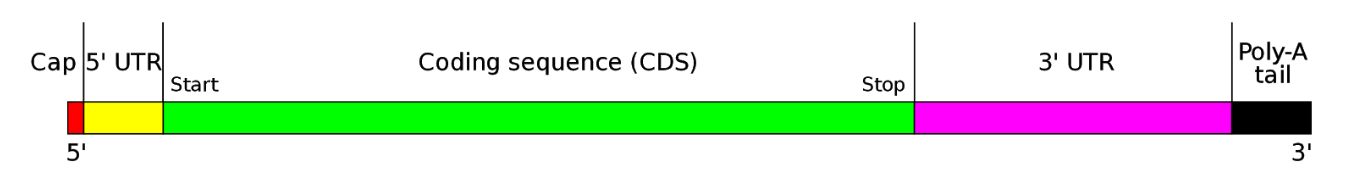
\includegraphics{https://raw.githubusercontent.com/LuchaoQi/JHU/master/Computational\%20Genomics\%20Applied\%20Comparativa\%20Genomics/hw1/1.png}

\paragraph{Codes used are shown here:}\label{codes-used-are-shown-here}

\begin{Shaded}
\begin{Highlighting}[]
\CommentTok{#!/usr/bin/env python3  }
\ImportTok{import}\NormalTok{ sys  }
\NormalTok{f }\OperatorTok{=}\NormalTok{ sys.stdin  }
\NormalTok{line }\OperatorTok{=}\NormalTok{ f.readline()  }
\NormalTok{dic }\OperatorTok{=}\NormalTok{ \{\}  }
\ControlFlowTok{while}\NormalTok{ line }\OperatorTok{!=} \StringTok{''}\NormalTok{:  }
\NormalTok{    line }\OperatorTok{=}\NormalTok{ line.strip().rstrip(}\StringTok{'}\CharTok{\textbackslash{}n}\StringTok{'}\NormalTok{).split()  }
\NormalTok{    dic[line[}\DecValTok{0}\NormalTok{]]}\OperatorTok{=}\BuiltInTok{int}\NormalTok{(line[}\DecValTok{1}\NormalTok{])  }
     \CommentTok{###int is really really really important!!!!  }
\NormalTok{    line }\OperatorTok{=}\NormalTok{ f.readline()  }
\NormalTok{f.close()  }
\BuiltInTok{print}\NormalTok{(}\StringTok{'number of chromosomes:'}\NormalTok{,}\BuiltInTok{len}\NormalTok{(dic))  }
  
\NormalTok{n }\OperatorTok{=} \DecValTok{0}  
\ControlFlowTok{for}\NormalTok{ i }\KeywordTok{in}\NormalTok{ dic:  }
\NormalTok{    n }\OperatorTok{+=} \BuiltInTok{int}\NormalTok{(dic[i])  }
\BuiltInTok{print}\NormalTok{(}\StringTok{'total length:'}\NormalTok{,n)  }
  
\NormalTok{b }\OperatorTok{=} \BuiltInTok{max}\NormalTok{(dic.values())   }\CommentTok{# largest size  }
\NormalTok{c }\OperatorTok{=} \BuiltInTok{list}\NormalTok{(dic.keys())[}\BuiltInTok{list}\NormalTok{(dic.values()).index(b)]   }\CommentTok{#coresponding name  }
\BuiltInTok{print}\NormalTok{(}\StringTok{'largest chromosome size and name: }\SpecialCharTok{%s}\StringTok{ }\SpecialCharTok\NormalTok{(c,b))  }
  
\NormalTok{b }\OperatorTok{=} \BuiltInTok{min}\NormalTok{(dic.values())   }\CommentTok{# smallest size  }
\NormalTok{c }\OperatorTok{=} \BuiltInTok{list}\NormalTok{(dic.keys())[}\BuiltInTok{list}\NormalTok{(dic.values()).index(b)]       }\CommentTok{#coresponding name  }
\BuiltInTok{print}\NormalTok{(}\StringTok{'smallest chromosome size and name: }\SpecialCharTok{%s}\StringTok{ }\SpecialCharTok\NormalTok{(c,b))  }
  
\BuiltInTok{print}\NormalTok{(}\StringTok{'mean chromosome length:'}\NormalTok{,}\BuiltInTok{format}\NormalTok{(n}\OperatorTok{/}\BuiltInTok{len}\NormalTok{(dic),}\StringTok{'.1f'}\NormalTok{))  }
\end{Highlighting}
\end{Shaded}

\subsubsection{Question 2: Sequence
content}\label{question-2-sequence-content}

Download the yeast genome from here:
\url{http://schatz-lab.org/appliedgenomics2019/assignments/assignment1/yeast.fa.gz}

\begin{itemize}
\tightlist
\item
  Question 2.1. How many As, Cs, Gs, Ts are found in the entire genome
\item
  Question 2.2. Make a scatterplot of the \%GC of 100bp windows across
  the genome: x-axis = genome location, y-axis = (\#G + \#C) / 100. For
  this analysis the chromsomes can be concatenated together to form a
  long string of the chromosomes in numerical order: chr1, chr2,
  \ldots{} chrN. Make sure to draw a bar to indicate the ends of
  chromosomes
\item
  Question 2.3. Make a histogram of the number of genomic bins of a
  given \%GC: x-axis = \%GC, y-axis = \# genomic bins with this \%GC
\item
  Question 2.4. Recall that Illumina sequencing performs poorly when the
  \%GC is \textless{}= 30\% or \textgreater{}= 65\%. Based on the
  analysis from Q2.2, what fraction of the genome do you expect to
  sequence poorly?
\end{itemize}

\paragraph{Answers:}\label{answers-1}

\subparagraph{Question 2.1.}\label{question-2.1.}

Silimar solutions in Q1, count the number of As, Cs, Gs, Ts in the
entire genome using str.count()\\
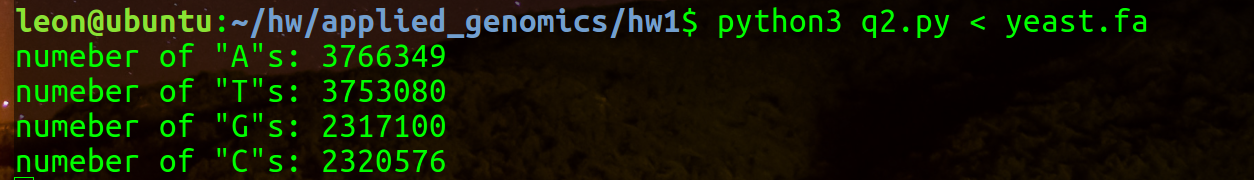
\includegraphics{https://raw.githubusercontent.com/LuchaoQi/JHU/master/Computational\%20Genomics\%20Applied\%20Comparativa\%20Genomics/hw1/Capture.PNG}

\subparagraph{Question 2.2.}\label{question-2.2.}

Using a dictionary whith key equals \# of window, value equals \%GC and
draw this distionary:\\
\includegraphics{https://raw.githubusercontent.com/LuchaoQi/hw/master/applied_genomics/hw1/figure_1.png}

\subparagraph{Question 2.3.}\label{question-2.3.}

Count the number of multiple values responding to one key and draw the
bar:\\
\includegraphics{https://raw.githubusercontent.com/LuchaoQi/hw/master/applied_genomics/hw1/figure_1-1.png}

\subparagraph{Question 2.4.}\label{question-2.4.}

From the results shown in Q2.2, we could expect windows arround \#32000,
\#33000 would perform poorly.

\paragraph{Codes used are shown
here:}\label{codes-used-are-shown-here-1}

\begin{Shaded}
\begin{Highlighting}[]
\CommentTok{#!/usr/bin/env python3}
\ImportTok{import}\NormalTok{ sys, matplotlib.pyplot }\ImportTok{as}\NormalTok{ plt}
\NormalTok{f }\OperatorTok{=}\NormalTok{ sys.stdin}
\NormalTok{line }\OperatorTok{=}\NormalTok{ sys.stdin.readline() }\CommentTok{#skip header}
\NormalTok{line }\OperatorTok{=}\NormalTok{ sys.stdin.readline()}
\NormalTok{seq }\OperatorTok{=} \StringTok{''}
\ControlFlowTok{while}\NormalTok{ line }\OperatorTok{!=} \StringTok{''}\NormalTok{:}
\NormalTok{    seq }\OperatorTok{+=}\NormalTok{ line.strip().rstrip(}\StringTok{'}\CharTok{\textbackslash{}n}\StringTok{'}\NormalTok{)}
\NormalTok{    line }\OperatorTok{=}\NormalTok{ f.readline()}
\NormalTok{f.close()}
\BuiltInTok{print}\NormalTok{(}\StringTok{'numeber of "'"A"'"s:'}\NormalTok{, seq.count(}\StringTok{'A'}\NormalTok{))}
\BuiltInTok{print}\NormalTok{(}\StringTok{'numeber of "'"T"'"s:'}\NormalTok{, seq.count(}\StringTok{'T'}\NormalTok{))}
\BuiltInTok{print}\NormalTok{(}\StringTok{'numeber of "'"G"'"s:'}\NormalTok{, seq.count(}\StringTok{'G'}\NormalTok{))}
\BuiltInTok{print}\NormalTok{(}\StringTok{'numeber of "'"C"'"s:'}\NormalTok{, seq.count(}\StringTok{'C'}\NormalTok{))}
\CommentTok{### Question 2.2}
\NormalTok{n }\OperatorTok{=} \BuiltInTok{len}\NormalTok{(seq)}\OperatorTok{//}\DecValTok{100}    \CommentTok{#number of bins, discard the last window   }
\NormalTok{dic }\OperatorTok{=}\NormalTok{\{\}}
\ControlFlowTok{for}\NormalTok{ i }\KeywordTok{in} \BuiltInTok{range}\NormalTok{(n):}
\NormalTok{    b }\OperatorTok{=} \StringTok{''}
\NormalTok{    b }\OperatorTok{+=}\NormalTok{ seq[}\DecValTok{100}\OperatorTok{*}\NormalTok{i:}\DecValTok{100}\OperatorTok{*}\NormalTok{(i}\OperatorTok{+}\DecValTok{1}\NormalTok{)] }\CommentTok{#divide the sequence by a window of 100}
    \ControlFlowTok{for}\NormalTok{ x }\KeywordTok{in}\NormalTok{ b:     }\CommentTok{#for each bin, count #GC}
\NormalTok{        gc }\OperatorTok{=} \StringTok{''}
\NormalTok{        gc }\OperatorTok{+=} \BuiltInTok{str}\NormalTok{(b.count(}\StringTok{'G'}\NormalTok{)}\OperatorTok{+}\NormalTok{b.count(}\StringTok{'C'}\NormalTok{))}
\NormalTok{    dic[i}\OperatorTok{+}\DecValTok{1}\NormalTok{]}\OperatorTok{=} \BuiltInTok{int}\NormalTok{(gc)}\OperatorTok{/}\DecValTok{100}   \CommentTok{# get a dictionary: key is the number of   \textbackslash{}window, value is %GC}
\CommentTok{###Q2.2###}
\NormalTok{lists }\OperatorTok{=} \BuiltInTok{sorted}\NormalTok{(dic.items())}
\NormalTok{x,y }\OperatorTok{=} \BuiltInTok{zip}\NormalTok{(}\OperatorTok{*}\NormalTok{lists)}
\NormalTok{plt.scatter(x,y)}
\NormalTok{plt.suptitle(}\StringTok{'}\SpecialCharTok{%G}\StringTok{C of 100bp windows across the genome'}\NormalTok{,fontsize }\OperatorTok{=} \DecValTok{30}\NormalTok{)}
\NormalTok{plt.xlabel(}\StringTok{'# of 100bp windows'}\NormalTok{,fontsize }\OperatorTok{=} \DecValTok{25}\NormalTok{)}
\NormalTok{plt.ylabel(}\StringTok{'}\SpecialCharTok{% o}\StringTok{f G+C'}\NormalTok{,fontsize }\OperatorTok{=} \DecValTok{25}\NormalTok{)}
\NormalTok{plt.xlim(}\DecValTok{0}\OperatorTok{-}\DecValTok{10000}\NormalTok{,}\BuiltInTok{max}\NormalTok{(x)}\OperatorTok{+}\DecValTok{10000}\NormalTok{)}
\NormalTok{plt.ylim(}\DecValTok{0}\NormalTok{,}\DecValTok{1}\NormalTok{)}
\NormalTok{plt.vlines(}\BuiltInTok{max}\NormalTok{(x),}\DecValTok{0}\NormalTok{,}\DecValTok{1}\NormalTok{)}
\NormalTok{plt.annotate(}\StringTok{' End of chromosome:}\CharTok{\textbackslash{}n}\StringTok{ discard the last window }\CharTok{\textbackslash{}n}\StringTok{ which is less than 100bp'}\NormalTok{,(}\BuiltInTok{max}\NormalTok{(x),}\FloatTok{0.4}\NormalTok{),fontsize }\OperatorTok{=} \DecValTok{25}\NormalTok{)}
\NormalTok{plt.show()}
\CommentTok{###Q2.3###}
\ControlFlowTok{for}\NormalTok{ i }\KeywordTok{in} \BuiltInTok{range}\NormalTok{(n):}
\NormalTok{    b }\OperatorTok{=} \StringTok{''}
\NormalTok{    b }\OperatorTok{+=}\NormalTok{ seq[}\DecValTok{100}\OperatorTok{*}\NormalTok{i:}\DecValTok{100}\OperatorTok{*}\NormalTok{(i}\OperatorTok{+}\DecValTok{1}\NormalTok{)]}
    \ControlFlowTok{for}\NormalTok{ x }\KeywordTok{in}\NormalTok{ b:}
\NormalTok{        gc }\OperatorTok{=} \StringTok{''}
\NormalTok{        gc }\OperatorTok{+=} \BuiltInTok{str}\NormalTok{(b.count(}\StringTok{'G'}\NormalTok{)}\OperatorTok{+}\NormalTok{b.count(}\StringTok{'C'}\NormalTok{))}
\NormalTok{    dic[i}\OperatorTok{+}\DecValTok{1}\NormalTok{]}\OperatorTok{=} \BuiltInTok{int}\NormalTok{(gc)}
\NormalTok{dic1}\OperatorTok{=}\NormalTok{\{\}}
\ControlFlowTok{for}\NormalTok{ n }\KeywordTok{in} \BuiltInTok{range}\NormalTok{(}\DecValTok{101}\NormalTok{):}
\NormalTok{    dic1[n]}\OperatorTok{=}\BuiltInTok{sum}\NormalTok{(value }\OperatorTok{==}\NormalTok{ n }\ControlFlowTok{for}\NormalTok{ value }\KeywordTok{in}\NormalTok{ dic.values())}
\CommentTok{#print(dic1)}
\NormalTok{plt.suptitle(}\StringTok{'Question 2.3'}\NormalTok{,fontsize }\OperatorTok{=} \DecValTok{30}\NormalTok{)}
\NormalTok{lists }\OperatorTok{=} \BuiltInTok{sorted}\NormalTok{(dic1.items())}
\NormalTok{x,y }\OperatorTok{=} \BuiltInTok{zip}\NormalTok{(}\OperatorTok{*}\NormalTok{lists)}
\NormalTok{plt.bar(x,y)}
\NormalTok{plt.xlabel(}\StringTok{'}\SpecialCharTok{%G}\StringTok{C*100'}\NormalTok{,fontsize }\OperatorTok{=} \DecValTok{25}\NormalTok{)}
\NormalTok{plt.ylabel(}\StringTok{'# of windows with coresponding }\SpecialCharTok{%G}\StringTok{C'}\NormalTok{,fontsize }\OperatorTok{=} \DecValTok{25}\NormalTok{)}
\NormalTok{plt.show()}
\end{Highlighting}
\end{Shaded}


\end{document}
